% Options for packages loaded elsewhere
\PassOptionsToPackage{unicode}{hyperref}
\PassOptionsToPackage{hyphens}{url}
%
\documentclass[
  openany]{book}
\usepackage{amsmath,amssymb}
\usepackage{lmodern}
\usepackage{iftex}
\ifPDFTeX
  \usepackage[T1]{fontenc}
  \usepackage[utf8]{inputenc}
  \usepackage{textcomp} % provide euro and other symbols
\else % if luatex or xetex
  \usepackage{unicode-math}
  \defaultfontfeatures{Scale=MatchLowercase}
  \defaultfontfeatures[\rmfamily]{Ligatures=TeX,Scale=1}
\fi
% Use upquote if available, for straight quotes in verbatim environments
\IfFileExists{upquote.sty}{\usepackage{upquote}}{}
\IfFileExists{microtype.sty}{% use microtype if available
  \usepackage[]{microtype}
  \UseMicrotypeSet[protrusion]{basicmath} % disable protrusion for tt fonts
}{}
\makeatletter
\@ifundefined{KOMAClassName}{% if non-KOMA class
  \IfFileExists{parskip.sty}{%
    \usepackage{parskip}
  }{% else
    \setlength{\parindent}{0pt}
    \setlength{\parskip}{6pt plus 2pt minus 1pt}}
}{% if KOMA class
  \KOMAoptions{parskip=half}}
\makeatother
\usepackage{xcolor}
\IfFileExists{xurl.sty}{\usepackage{xurl}}{} % add URL line breaks if available
\IfFileExists{bookmark.sty}{\usepackage{bookmark}}{\usepackage{hyperref}}
\hypersetup{
  pdftitle={MSU I.O Student Mentorship Program User Manual},
  pdfauthor={Eagle I.O},
  hidelinks,
  pdfcreator={LaTeX via pandoc}}
\urlstyle{same} % disable monospaced font for URLs
\usepackage{longtable,booktabs,array}
\usepackage{calc} % for calculating minipage widths
% Correct order of tables after \paragraph or \subparagraph
\usepackage{etoolbox}
\makeatletter
\patchcmd\longtable{\par}{\if@noskipsec\mbox{}\fi\par}{}{}
\makeatother
% Allow footnotes in longtable head/foot
\IfFileExists{footnotehyper.sty}{\usepackage{footnotehyper}}{\usepackage{footnote}}
\makesavenoteenv{longtable}
\usepackage{graphicx}
\makeatletter
\def\maxwidth{\ifdim\Gin@nat@width>\linewidth\linewidth\else\Gin@nat@width\fi}
\def\maxheight{\ifdim\Gin@nat@height>\textheight\textheight\else\Gin@nat@height\fi}
\makeatother
% Scale images if necessary, so that they will not overflow the page
% margins by default, and it is still possible to overwrite the defaults
% using explicit options in \includegraphics[width, height, ...]{}
\setkeys{Gin}{width=\maxwidth,height=\maxheight,keepaspectratio}
% Set default figure placement to htbp
\makeatletter
\def\fps@figure{htbp}
\makeatother
\setlength{\emergencystretch}{3em} % prevent overfull lines
\providecommand{\tightlist}{%
  \setlength{\itemsep}{0pt}\setlength{\parskip}{0pt}}
\setcounter{secnumdepth}{5}
\usepackage{booktabs}
\usepackage{booktabs}
\usepackage{longtable}
\usepackage{array}
\usepackage{multirow}
\usepackage{wrapfig}
\usepackage{float}
\usepackage{colortbl}
\usepackage{pdflscape}
\usepackage{tabu}
\usepackage{threeparttable}
\usepackage{threeparttablex}
\usepackage[normalem]{ulem}
\usepackage{makecell}
\usepackage{xcolor}
\ifLuaTeX
  \usepackage{selnolig}  % disable illegal ligatures
\fi
\usepackage[]{natbib}
\bibliographystyle{plainnat}

\title{MSU I.O Student Mentorship Program User Manual}
\author{Eagle I.O}
\date{Most recent update 2022-05-23}

\begin{document}
\maketitle

{
\setcounter{tocdepth}{1}
\tableofcontents
}
\hypertarget{Homepage}{%
\chapter*{Homepage}\label{Homepage}}
\addcontentsline{toc}{chapter}{Homepage}

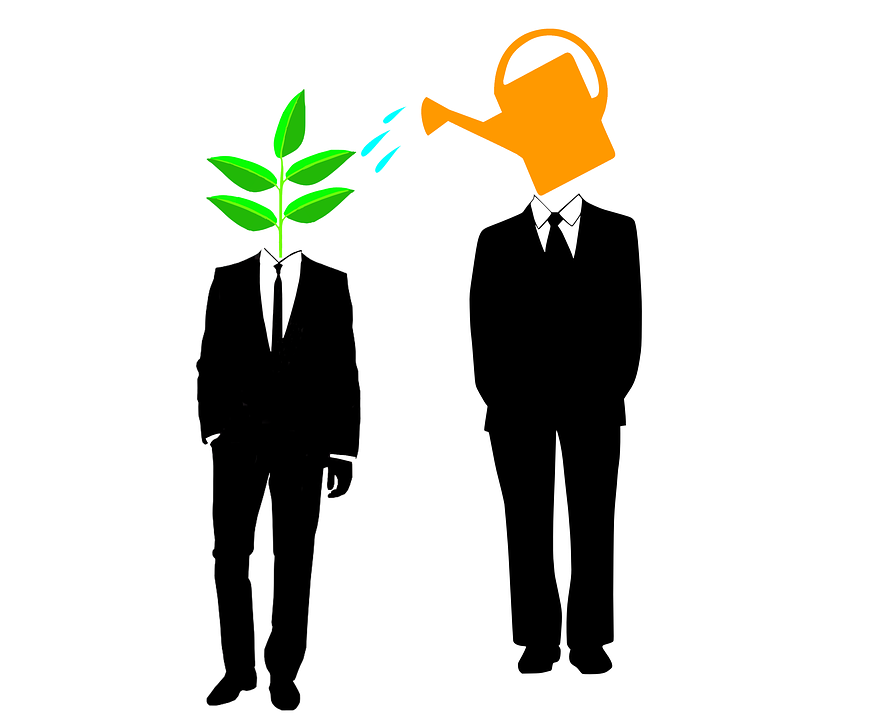
\includegraphics{images/cover.png}

This manual was written in \href{https://bookdown.org/}{\emph{Bookdown}} using the \href{https://bookdown.org/yihui/bookdown/html.html}{\emph{GitBook}} style.

\hypertarget{mentoring-overview}{%
\chapter{Mentoring Overview}\label{mentoring-overview}}


\includegraphics{images/greek.jpg}

\hypertarget{history-definition}{%
\section{History \& Definition}\label{history-definition}}

The meaning of the word ``Mentor'' has evolved to describe a person that facilitates personal and professional growth in an individual by sharing knowledge and insight that have been learned through the years. Mentoring is a relationship. In short, mentoring is a relationship between two individuals of different levels of experience, one senior and one junior in experience, that focuses on advancing professional and personal development. Mentoring is about information sharing and learning through and with another person. From Professor Dumbledore and Harry Potter to Socrates and Plato to Obi-Wan Kenobi and Luke Skywalker, it is clear mentoring relationships come in all shapes and sizes. Individual differences make no two mentoring relationships alike, but are all based on mutual trust, respect, and integrity.

\hypertarget{background}{%
\section{Background}\label{background}}

The Montclair State University Industrial and Organizational Psychology Graduate Program is proud to offer a Student Mentor Program for students in their first year of graduate school. Incoming students are matched with a mentor who can provide extracurricular support and share first-hand knowledge about the I.O profession. Incoming Masters students will be matched with either a returning Master's or Ph.D.~student, and incoming Ph.D.~students will only be paired with a returning Ph.D.~student. Mentor and mentee pairings are then made based upon mutual interests in I.O psychology.

\hypertarget{mission-statement}{%
\section{Mission Statement}\label{mission-statement}}

Our mentor program is dedicated to creating an environment that fosters growth, development, and engagement of first year I.O students to become successful academically, professionally, and socially during graduate school.

\hypertarget{why-join}{%
\chapter{Why Join?}\label{why-join}}


\includegraphics{images/why.jpeg}

\hypertarget{benefits-for-mentees}{%
\section{Benefits for Mentees}\label{benefits-for-mentees}}

Working with a mentor can be an advantage for an incoming student. Mentees gain valuable experience by forging one-on-one relationships with current I.O graduate students. These experiences include:

\begin{itemize}
\tightlist
\item
  Help with setting realistic goals.
\item
  Strengthening knowledge of the industry, organizational culture, and job functions.
\item
  Expanding your existing network and support system.
\item
  Receiving feedback from an experienced student.
\item
  Enhancing overall professional effectiveness.
\item
  Gaining knowledge and experience to be a future mentor.
\end{itemize}

\hypertarget{benefits-for-mentors}{%
\section{Benefits for Mentors}\label{benefits-for-mentors}}

Contributing time and expertise as a mentor is a valuable way to give back and foster the next generation of MSU I.O Psychology graduate students. Mentoring can be both personally and professionally rewarding, as mentors learn the value in helping their peers succeed. Some benefits of being a mentor include:

\begin{itemize}
\tightlist
\item
  Build leadership skills.
\item
  Build communication skills.
\item
  Expand professional network and increase visibility.
\item
  Contribute to the advancement of the profession.
\end{itemize}

\hypertarget{responsibilities}{%
\chapter{Responsibilities}\label{responsibilities}}


\includegraphics{images/responsibility.jpg}

The key to success for students is to commit time and effort toward developing their future careers by taking full advantage of this unique opportunity. Mentees should supply their mentor with feedback and be open to receiving advice and coaching from the mentor.

\hypertarget{mentee-expectations}{%
\section{Mentee Expectations}\label{mentee-expectations}}

\begin{itemize}
\tightlist
\item
  Be accountable for upholding commitment to the mentorship program.
\item
  Determine your goals and discuss these with your mentor.
\item
  Attend at least one activity each semester (see Chapter \ref{timeline} for a calendar of events).
\item
  Attend at least one networking event per semester.
\item
  Ask for help and guidance; seek out the information needed for your career development.
\item
  Communicate any academic concerns that you might want assistance working through.
\item
  Communicate any concerns you have in transitioning from the program into the workforce.
\item
  Accept both praise and constructive criticism.
\item
  Determine acceptable time and format to communicate.
\item
  Uphold Montclair State University's \href{https://www.montclair.edu/policies/all-policies/academic-honesty-and-integrity/}{Academic Honesty and Integrity Policy}.
\end{itemize}

\emph{If you wish to opt out of the mentoring program}, please contact our \href{mailto:simonetd@montclair.edu}{program director}.

\hypertarget{student-mentor-expectations}{%
\section{Student Mentor Expectations}\label{student-mentor-expectations}}

Mentors take a leadership role within the Mentorship program, they are meant to provide guidance and support to incoming members of the Industrial and Organizational Psychology program.\footnote{Mentors participate in the program willingly, but once they commit to participating in the program they need to stay on board for the remainder of the year unless there is an emergent situation. If mentors plan on leaving the program they need to communicate this to Eagle I.O as soon as possible so that arrangements can be made for the following semester.}

\begin{itemize}
\tightlist
\item
  Attend MSU I.O Program orientation (see Chapter \ref{timeline}).
\item
  Work with the mentee in developing an Individual Development Plan (IDP; Chapter \ref{sdp}) using:

  \begin{itemize}
  \tightlist
  \item
    Goal setting (\href{https://piximus.net/media/12860/funny-demotivational-posters-86-28.jpg}{Utilize goal setting theories}): help mentee set goals for the semester; academic, personal, professional, and social.
  \item
    Motivational theory (\href{https://youtu.be/cgg9byUy-V4}{Utilize Motivation theories}).
  \end{itemize}
\item
  Mentors must attend at least one networking event per semester.
\item
  Stay accessible, committed, and engaged during the length of the program.\\
\item
  Setting and agreeing on frequency of meeting times according to needs/wants/availability.

  \begin{itemize}
  \tightlist
  \item
    In-person meet-ups
  \item
    Over the phone ``meet-ups''
  \item
    Zoom `meet-ups'
  \item
    Being accessible to mentee when help is needed, and encourage mentee to attend office hours when they need help and the mentor is not available.
  \end{itemize}
\item
  Addressing boundaries related to academic support.

  \begin{itemize}
  \tightlist
  \item
    Time frame to request and provide help such as hours and days available.
  \item
    Boundaries regarding personal information provided (cell number, personal email, etc).
  \item
    What type of academic support is okay to request and provide.
  \end{itemize}
\item
  Inform mentees about the importance of networking and extracurricular events.

  \begin{itemize}
  \tightlist
  \item
    Encourage mentees to attend developmental events outside the program (for example, \href{http://www.siop.org}{SIOP}, monthly \href{http://www.metroapppsych.com/}{METROs}, Career/job fairs, ect.). More information about this will be provided through the event calendar (Chapter \ref{timeline}).
  \item
    Provide support getting to events, such as METRO and career fairs (if possible).
  \end{itemize}
\item
  Cultivate professionalism:

  \begin{itemize}
  \tightlist
  \item
    Mentor should help mentee search and prepare for internship opportunities (if needed by mentee).
  \item
    Mentors should model professional behavior to set the example for mentees.
  \end{itemize}
\item
  Uphold Montclair State University's \href{https://www.montclair.edu/policies/all-policies/academic-honesty-and-integrity/}{Academic Honesty and Integrity Policy}
\item
  If mentor has any questions or concerns that may arise, let Eagle I.O know to be able to provide support and guidance.

  \begin{itemize}
  \tightlist
  \item
    \emph{If you have any issues}, please contact \href{mailto:eagleio@montclair.edu}{Eagle IO}.
  \end{itemize}
\end{itemize}

\hypertarget{aumni-mentor-expectations}{%
\section{Aumni Mentor Expectations}\label{aumni-mentor-expectations}}

Alumni mentors are present to provide guidance and support in relation to the transition from school to work. They provide tips and suggestions for networking building, starting new positions, and applying to positions. Alumni mentors are not responsbile nor required to provide their mentees with positions in the workforce; however, they are expected to advise their mentees when pursuing new positions or have questions regarding their current role.\footnote{Mentors participate in the program willingly, but once they commit to participating in the program they need to stay on board for the remainder of the year unless there is an emergent situation. If mentors plan on leaving the program they need to communicate this to Eagle I.O as soon as possible so that arrangements can be made for the following semester.}

\begin{itemize}
\tightlist
\item
  Help mentee set goals for the semester:

  \begin{itemize}
  \tightlist
  \item
    Academic, personal, professional, and social.
  \item
    Motivational theory (\href{https://youtu.be/cgg9byUy-V4}{Utilize Motivation theories})
  \end{itemize}
\item
  Mentors are encouraged but not required to attend at least one networking event per semester.
\item
  Stay accessible, committed, and engaged during the length of their commitment to the mentorship program.
\item
  Setting and agreeing on frequency of meeting times according to needs/wants/.

  \begin{itemize}
  \tightlist
  \item
    In-person meet-ups
  \item
    Over the phone ``meet-ups''
  \item
    Zoom `meet-ups'
  \item
    Being accessible to mentee when help is needed, and encourage mentee to attend a professor's office hours when they need help and the mentor is not available.
  \end{itemize}
\item
  Addressing boundaries related to academic and professional support.

  \begin{itemize}
  \tightlist
  \item
    Time frame to request and provide help such as hours and days available.
  \item
    Boundaries regarding personal information provided (cell number, personal email, etc).
  \item
    What type of academic and professional support is okay to request and provide.
  \end{itemize}
\item
  Inform mentees about the importance of networking and extracurricular events.

  \begin{itemize}
  \tightlist
  \item
    Encourage mentees to attend developmental events outside the program (for example, \href{http://www.siop.org}{SIOP}, monthly \href{http://www.metroapppsych.com/}{METROs}, Career/job fairs, ect.). More information about this will be provided through the event calendar (Chapter \ref{timeline}).
  \end{itemize}
\item
  Cultivate professionalism

  \begin{itemize}
  \tightlist
  \item
    Mentor can help mentee search and prepare for internship and career opportunities (if needed by mentee).
  \item
    Mentors should model professional behavior to set the example for mentees.
  \end{itemize}
\item
  Uphold Montclair State University's \href{https://www.montclair.edu/policies/all-policies/academic-honesty-and-integrity/}{Academic Honesty and Integrity Policy}
\item
  If mentor has any questions or concerns that may arise, let Eagle I.O know to be able to provide support and guidance.

  \begin{itemize}
  \tightlist
  \item
    \emph{If you have any issues}, please contact \href{mailto:eagleio@montclair.edu}{Eagle IO}.
  \end{itemize}
\end{itemize}

\hypertarget{Eagle}{%
\section{Eagle I.O Roles and Responsibilities}\label{Eagle}}

\begin{itemize}
\tightlist
\item
  Ensure the mentoring program is created and sustained (see Chapter \ref{procedure} for outline).

  \begin{itemize}
  \tightlist
  \item
    Focus on succession planning within the group.
  \end{itemize}
\item
  Populate the calendar of Industrial-Organizational Psychology program related events. (\href{http://www.metroapppsych.com/}{METRO}, \href{http://www.siop.org/}{SIOP}, see Chapters \ref{fall19} and \ref{spring20})\\
\item
  Plan New Student Orientation procedures, events, and necessary materials.
\item
  Meet regularly to discuss progress, concerns, or setbacks regarding the mentors, mentees, and the program, itself.
\item
  Utilize and update existing toolkit.
\end{itemize}

\hypertarget{timeline}{%
\chapter{Planned Events Calendar}\label{timeline}}


\includegraphics{images/calendar.png}

\hypertarget{fall19}{%
\section{2021-2022 Academic Year}\label{fall19}}

\begin{tabular}{l|l|l|l|l}
\hline
Event & Date & Time & Description & Location\\
\hline
Orientation & 8/30/2021 & 5:00-8:00 PM & Opportunity for incoming students to become more acquainted with each other, the mentors, and professors, and the campus. & On campus. S\\
\hline
Social & 8/30/2021 & 8:00-10:00 PM & Opportunity for incoming students to meet each other, the returning students, and professors. & Alexus Steakhouse \& Tavern (955 Valley Rd, Clifton, NJ)\\
\hline
Classes begin & 9/2/2021 & All day & First day of classes. & Montclair State University\\
\hline
Labor Day holiday & 9/6/2021 & All day & No classes! & \\
\hline
Mentor/Mentee Check-in & 9/27/2021 & All day & Monthly reminder for mentors and mentees to contact one another & \\
\hline
SIOP Leading Edge Consortium Workshops & 9/30/2021-10/2/2021 & Various times & Topics related to leadership development. & Online\\
\hline
SIOP Leading Edge Consortium Workshops & 10/7/2021-10/9/2021 & Varous times & Topics related to leadership development. & Online\\
\hline
Mentor/Mentee Check-in & 10/22/2021 & All day & Monthly reminder for mentors and mentees to contact one another & \\
\hline
ILA Reimagining Leadership Together Conference & 10/24/2021-10/25/2021 & Various times & A conference geared towards leadership topics. & Online\\
\hline
SHRM Inclusion 2021 Conference & 10/25/2021-10/27/2021 & All day & A conferenced focused on diversity and inclusion topics. & Online and in person (Austin, TX)\\
\hline
Mentor/Mentee Check-in & 11/22/2021 & All day & Monthly reminder for mentors and mentees to contact one another & \\
\hline
Thanksgiving holiday & 11/25/2021-11/28/2021 &  & No classes! & \\
\hline
Last day of classes & 12/20/2021 &  & No classes! & \\
\hline
Career Workshop & TBD & TBD & An open event from the internship class. & On Campus and Zoom: TBD\\
\hline
Guest Speaker Event & TBD & TBD & An open event from the internship class. & On Campus and Zoom: TBD\\
\hline
Career Workshop & TBD & TBD & An open event from the internship class. & On Campus and Zoom: TBD\\
\hline
Goal-Setting Workshop & TBD & TBD & An event for mentors and mentees to discuss their upcoming goals for the semester, academic year, and early career. & TBD\\
\hline
First day of spring semester & 1/18/2022 &  & First day of classes. & Montclair State University\\
\hline
Mentor/Mentee Check-in & 1/26/2021 & All day & Monthly reminder for mentors and mentees to contact one another & \\
\hline
Mentor/Mentee Check-in & 2/25/2021 & All day & Monthly reminder for mentors and mentees to contact one another & \\
\hline
Spring break & 3/7/2022-3/13/2022 &  & No classes! & \\
\hline
Mentor/Mentee Check-in & 3/25/2021 & All day & Monthly reminder for mentors and mentees to contact one another & \\
\hline
Pre-Conference Week & April 11 - 17 & TBD & SIOP & Virtual\\
\hline
Conference Week 1 & April 18 - 24 & TBD & SIOP & Virtual\\
\hline
Conference Week 2 & April 25 - May 1 & TBD & SIOP & Seattle\\
\hline
Post-Conference Week & May 2 - 8 & TBD & SIOP & Virtual\\
\hline
Last day of classes & 5/12/2022 &  & Summer break begins! & \\
\hline
Mentor/Mentee Check-in & 5/26/2021 & All day & Monthly reminder for mentors and mentees to contact one another & \\
\hline
SIOP is hosting the 2021 Leading Edge Consortium (LEC) on Leading Edge: Leadership Development to explore these crucial business challenges. &  &  &  & \\
\hline
\end{tabular}

\hypertarget{procedure}{%
\chapter{Program Roll-Out}\label{procedure}}


\includegraphics{images/manage.jpg}

This page primarily serves as a procedural overview, so future Eagle I.O cohorts can implement and manage the Mentorship program.

Procedurally, Eagle I.O members:

\begin{enumerate}
\def\labelenumi{\arabic{enumi})}
\tightlist
\item
  Guage interest and availability via administering a \href{https://survey.az1.qualtrics.com/jfe/form/SV_1TFZ0AIYBpsyh6Z}{survey} sent by the program director in July

  \begin{itemize}
  \tightlist
  \item
    Several follow-up attempts are made during the summer
  \item
    Template documents:\footnote{Note these documents are only available to individuals who have an e-mail address with the ``montclair.edu'' domain}

    \begin{itemize}
    \tightlist
    \item
      \href{https://drive.google.com/open?id=1oDPE6IKPpk-vFezMzAU6uGP9HiTDfH4DSmJT1TQdXYU}{To Mentors}\\
    \item
      \href{https://drive.google.com/open?id=1BWLyBbBIcMEBeRxTNhBaLzbWkEPXThcO44qSh4HwTpw}{To First Year Mentees}\\
    \item
      \href{https://docs.google.com/document/d/1o_W0KReXqGGoR6jn1zabX6syhJ2sNjMZH8RPBwtfbnI/edit?usp=sharing}{First Two Events}
    \item
      \href{https://docs.google.com/document/d/1pGMk17GrXaWcjsuM3HTSouYSGxK_JAm5UVDu6EI7lI0/edit}{Alumni Recruitment}
    \end{itemize}
  \end{itemize}
\item
  Eagle I.O consultants match interested mentors and mentees

  \begin{itemize}
  \tightlist
  \item
    This is done prior to orientation
  \end{itemize}
\item
  Matches are introduced before orientation by email and discuss future events (see Chapter \ref{timeline})
\item
  The program is monitored periodically (see Chapter \ref{Eagle} ``Eagle I.O Responsibilities'')
\end{enumerate}

\hypertarget{fall20}{%
\section{Responsibility Calendar (Fall 2021)}\label{fall20}}

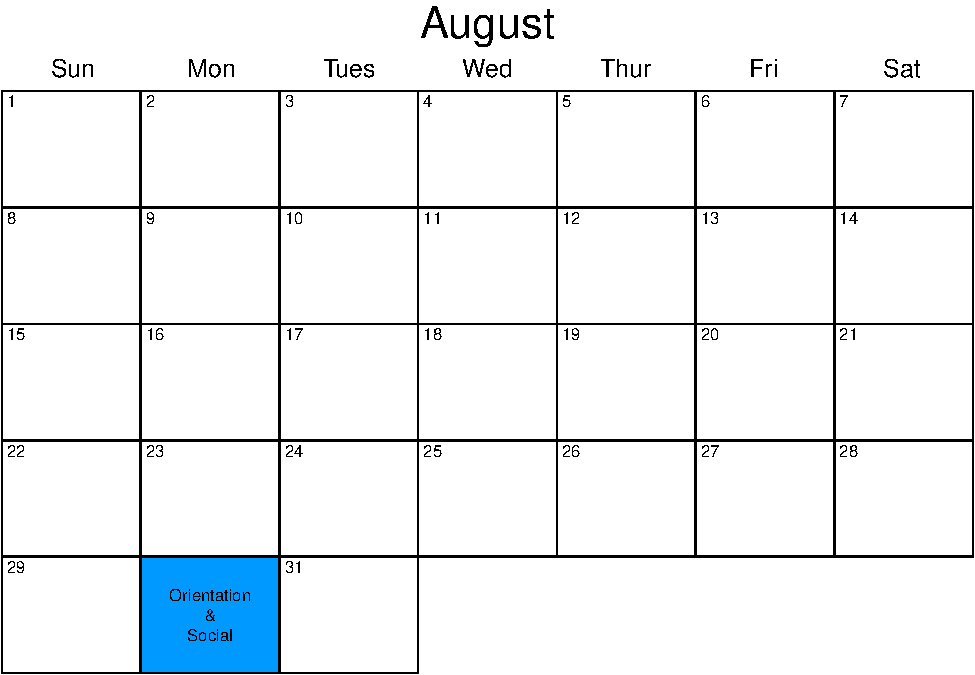
\includegraphics{_main_files/figure-latex/Fall2020-1.pdf} 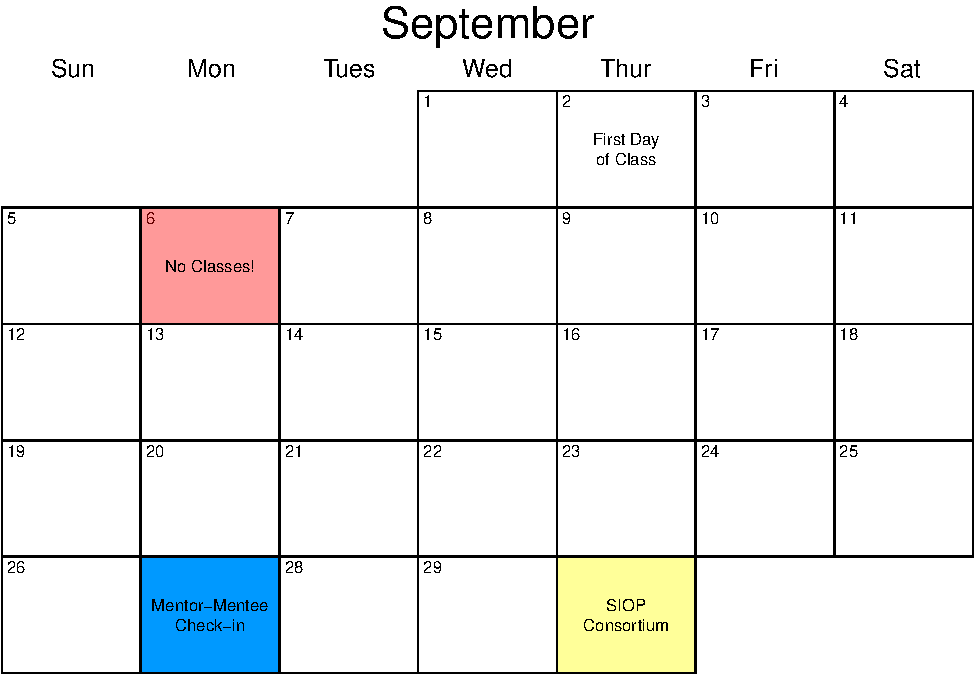
\includegraphics{_main_files/figure-latex/Fall2020-2.pdf} 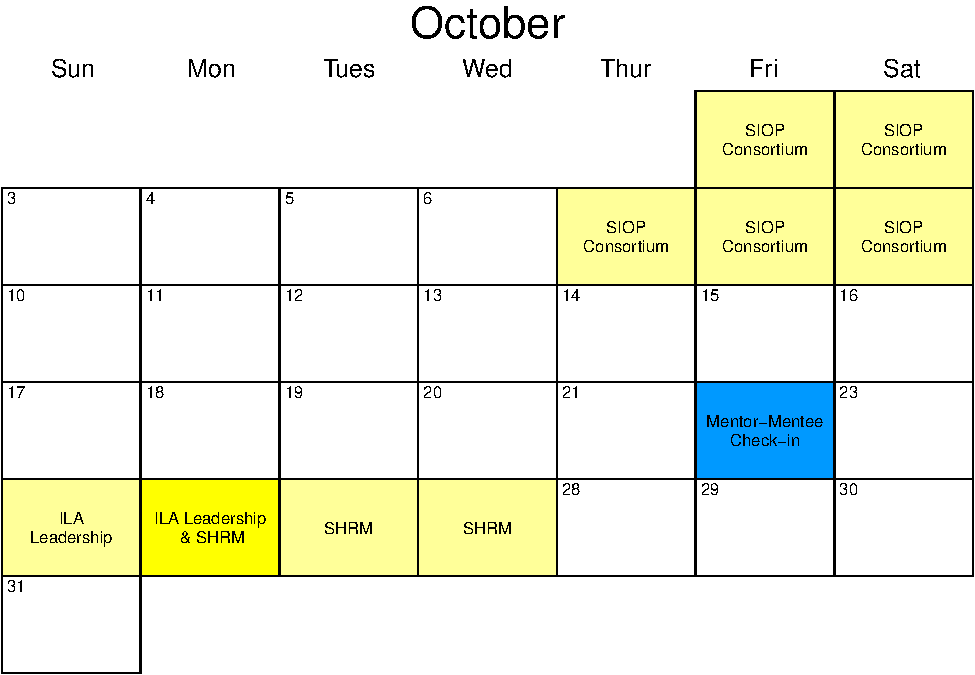
\includegraphics{_main_files/figure-latex/Fall2020-3.pdf} 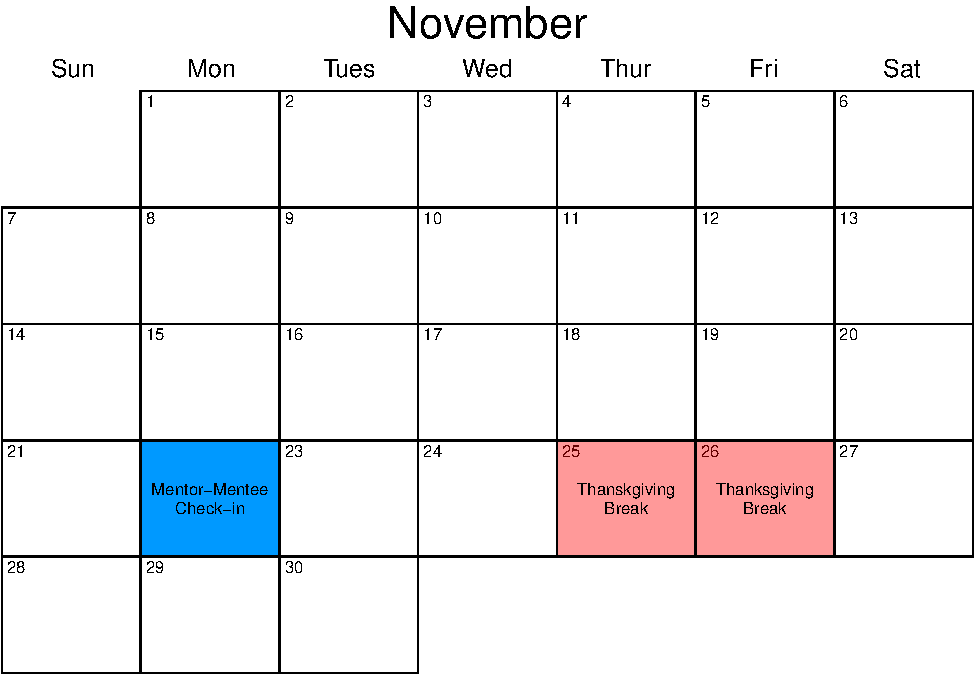
\includegraphics{_main_files/figure-latex/Fall2020-4.pdf} 
\includegraphics{_main_files/figure-latex/Fall2020-5.pdf}

\hypertarget{spring20}{%
\section{Responsibility Calendar (Spring 2022)}\label{spring20}}

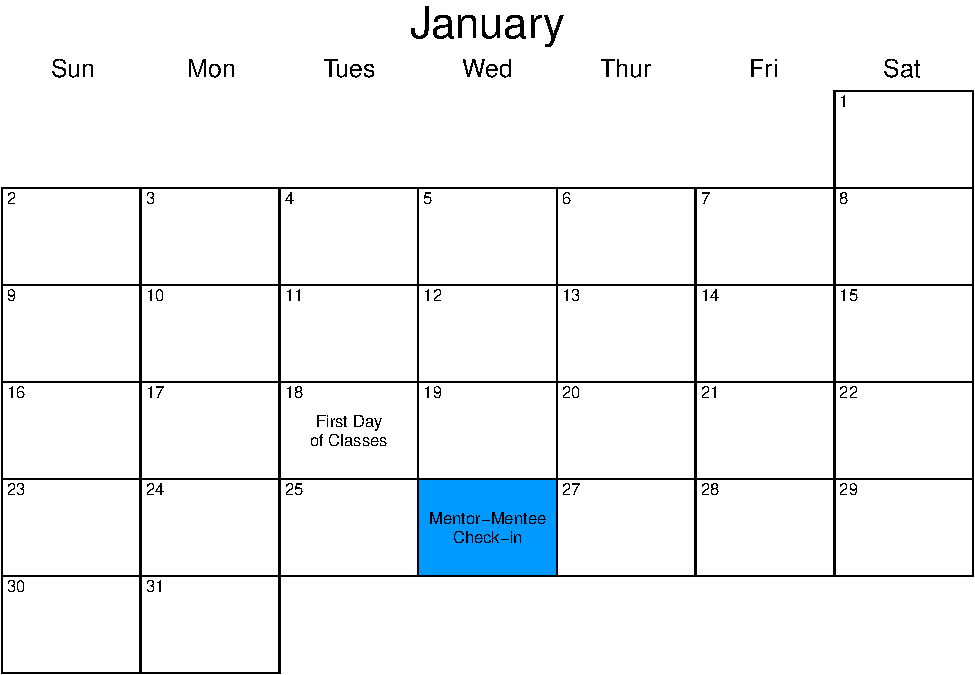
\includegraphics{_main_files/figure-latex/Spring2021-1.pdf} 
\includegraphics{_main_files/figure-latex/Spring2021-2.pdf} 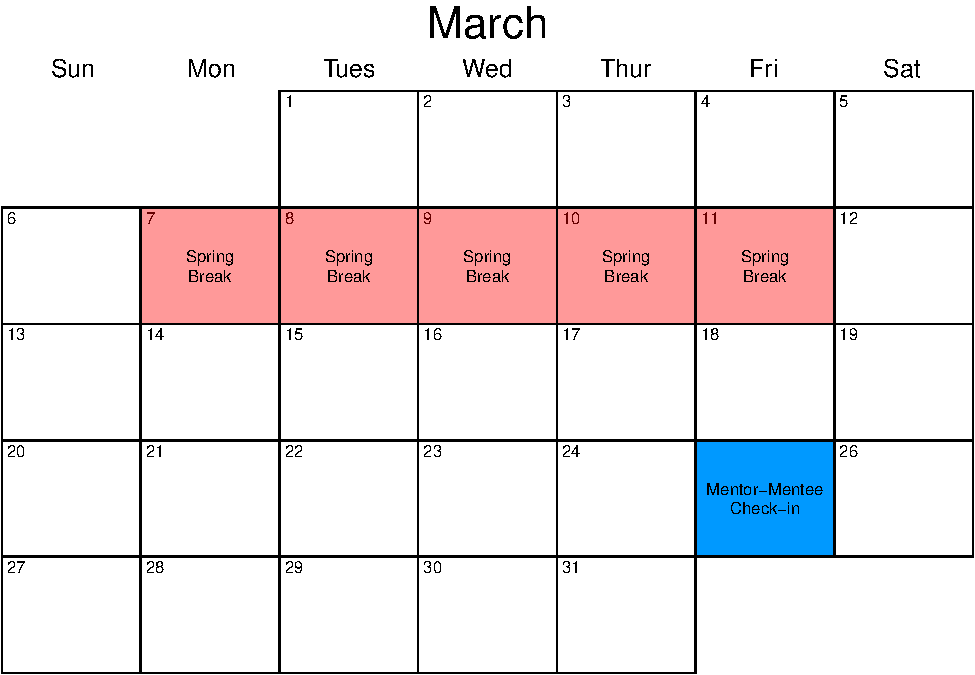
\includegraphics{_main_files/figure-latex/Spring2021-3.pdf} 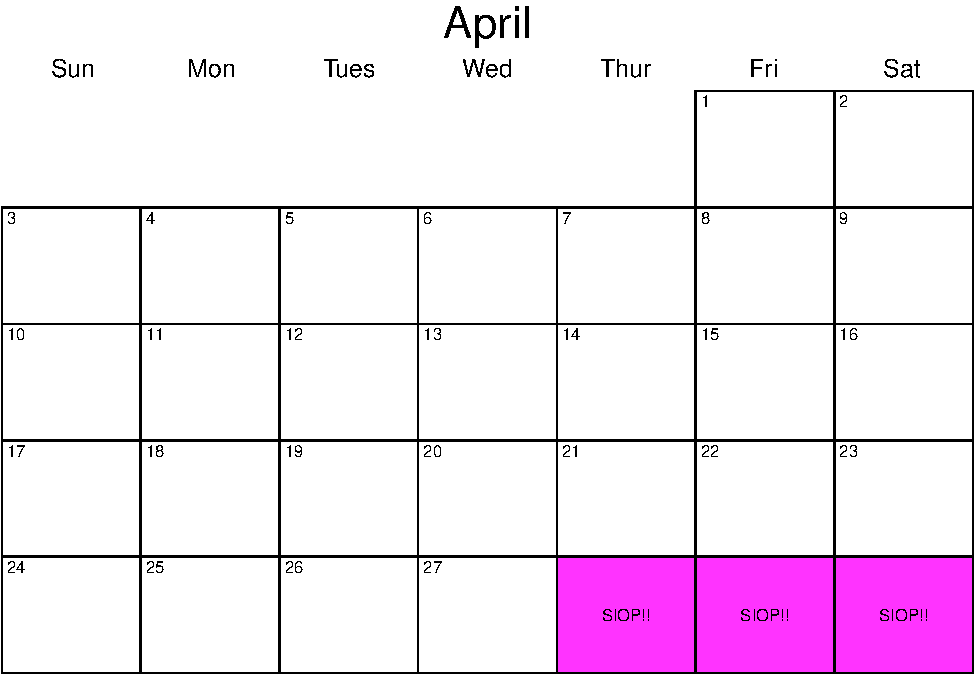
\includegraphics{_main_files/figure-latex/Spring2021-4.pdf} 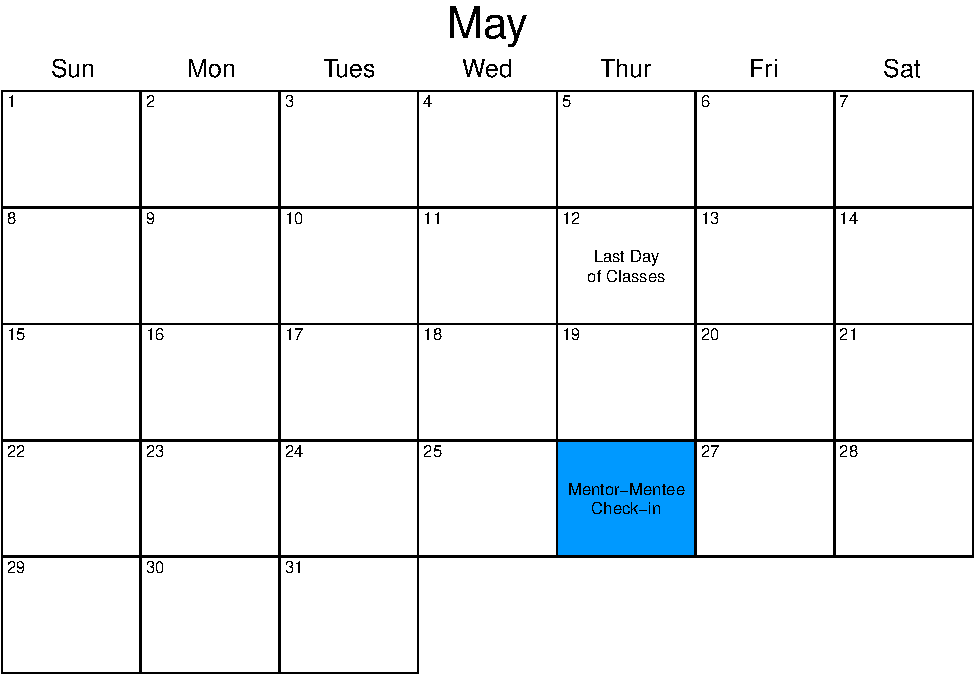
\includegraphics{_main_files/figure-latex/Spring2021-5.pdf}

\hypertarget{sdp}{%
\chapter{Individual Development Plan}\label{sdp}}


\includegraphics{images/idp.png}

This form will be completed at a manditory mid-Fall semester checkin and in mutual collaboration between the mentor and mentee.

In the event that the event cannot be held in person, mentor and mentee pairings will be required to meet virtually (see instructions to print this page below).

Mentee Top 3 Strengths:

\begin{enumerate}
\def\labelenumi{\arabic{enumi}.}
\tightlist
\item
\item
\item
\end{enumerate}

Mentee Top 3 Areas for Growth:

\begin{enumerate}
\def\labelenumi{\arabic{enumi}.}
\tightlist
\item
\item
\item
\end{enumerate}

Goals for the year:

\begin{enumerate}
\def\labelenumi{\arabic{enumi}.}
\tightlist
\item
\item
\item
\end{enumerate}

Action Plan:

\begin{enumerate}
\def\labelenumi{\arabic{enumi}.}
\tightlist
\item
\item
\item
\end{enumerate}

\hypertarget{standards-agreement}{%
\section{Standards Agreement}\label{standards-agreement}}

I hereby agree to follow my action plan\\

\begin{center}\rule{0.5\linewidth}{0.5pt}\end{center}

\textbf{Mentee}

\begin{center}\rule{0.5\linewidth}{0.5pt}\end{center}

\textbf{Mentor}

To print this page, please use the \href{snip.png}{``download icon'' and ``PDF'' options} available above.

\hypertarget{authors}{%
\chapter{About the Program Creators}\label{authors}}

Presented alphabetically:

\begin{tabular}{l|l}
\hline
![](sam.jpg) & [Samantha Biggs](mailto:biggss1@montclair.edu) received her BA in Psychology and a minor in French from Temple University (Class of 2018). Her I/O interests include Training and Development, Consulting, HR, and a lot of “O side” topics that she can’t pick (satisfaction, motivation, etc.)\\
\hline
[Renata Garcia Prieto Palacios Roji](mailto:garciaprier1@mail.montclair.edu) received her  BA in Psychology and minor in Philosophy from the University of Texas in 2017. Her I/O interests include Data analysis, Learning and Development, and Executive coaching. & ![](renata.png)\\
\hline
![](danielle.jpg) & [Danielle Granuzzo](mailto:granuzzod1@montclair.edu) received her B.A. In Psychology with a minor in Business from Ramapo College of New Jersey in 2018. Her I/O interests include Leadership/Organizational development, succession planning, learning and development, and change management.\\
\hline
[Taylor Jones](mailto:jonest26@montclair.edu) recieved her undergraduate degree in Psychology with minors in cognitive science and criminal justice (Marist College class of 2018). Her I/O interests include: learning and development, talent management,  leadership development, and AI and I-O & ![](taylor.jpg)\\
\hline
![](dehlia.jpg) & [Dehlia Mahoney](mailto:mahoneyd5@montclair.edu) received her undergraduate degree in Psychology from CUNY Queens College in 2017. Her I/O interests include  Servant-Leadership, Diversity \& Inclusion, Leadership Development, and Personnel Selection \& Assessment.\\
\hline
[Nishi Patel](mailto:pateln70@montclair.edu) received her Bachelor’s of Arts in Psychology with minors in Business and Leadership Development through Civic Engagement at Montclair State University in 2018. Her I/O interests include Talent Management, Learning and Development, Leadership in Organizations, Consultancy, and Human Resources. & ![](nishi.jpg)\\
\hline
![](elese.jpg) & [Elese Rodriguez](mailto:rodriqueze32@montclair.edu) received her Bachelor of Arts in Psychology with a minor in Social Work from Montclair State University (2017). Her interests include Talent Acquisition, Consultancy, Learning and Development, and Human Resources.\\
\hline
[Kristina Stiger](mailto:stigerk1@montclair.edu) received her B.S. in Accounting with a minor in Management Information Systems at Indiana University of Pennsylvania (IUP) in 2013. Her I/O interests include Change-management, design thinking,
leadership, employee experience, and team building. & ![](kristina.jpg)\\
\hline
\end{tabular}


\includegraphics[width=0.35\textwidth,height=\textheight]{Office1.png}
\includegraphics[width=0.3\textwidth,height=\textheight]{Office2.png}
\includegraphics[width=0.3\textwidth,height=\textheight]{Office3.png}


\includegraphics[width=0.25\textwidth,height=\textheight]{Office4.png}
\includegraphics[width=0.45\textwidth,height=\textheight]{Office5.png}
\includegraphics[width=0.28\textwidth,height=\textheight]{Office6.png}


\includegraphics[width=0.25\textwidth,height=\textheight]{Office7.png}
\includegraphics[width=0.35\textwidth,height=\textheight]{Office8.png}

\begin{enumerate}
\def\labelenumi{\arabic{enumi}.}
\item
  Students are more likely to persist and graduate in settings that provide academic, social, and personal support. Support may be provided in structured forms such as in summer bridge programs {[}and{]} mentor programs. \citep{tinto_promoting_2003}
\item
  After one year of mentoring by faculty, students with mentors have higher GPAs and are more likely to stay in college compared to students who do not have mentors. \citep{campbell_faculty/student_1997}
\item
  Mentoring increased students' GPA, mentored students failed fewer courses, and mentored students were much more likely to be in good academic standing after one year of college than non-mentored students (88.5\% vs.~57.1\%). \citep{salinitri_effects_2005}
\item
  Mentored first year students are significantly more likely to return to college for a second year. \citep{terenzini_students_1996}
\item
  Having a mentor in college helps students with identity formation, coping skills, stress reduction, and persistence to graduation. \citep{bordes_mentoring_2005}
\item
  Mentored minority college students are twice as likely to persist as non-mentored minority students. They also have higher GPAs than non---mentored students. \citep{crisp_mentoring_2009}
\item
  Formal and informal mentoring programs are conducive to the transition, retention, and success of minority students in higher education. • Students who participate are much more satisfied with their college experience than those who did not participate in mentoring programs. • Establishing multiple levels of mentoring programs------faculty, peers, staff, and administrators------is important in providing success mechanisms for minority students. \citep{pope_community_2002}
\item
  Having a mentor in college helps students with identity formation, coping skills, stress reduction, and persistence to graduation. \citep{bordes_mentoring_2005}
\end{enumerate}

  \bibliography{book.bib,mentor.bib,packages.bib}

\end{document}
